\documentclass[screen]{../../../../sty/open-logic-book}
\usepackage[all]{nowidow}
\usepackage[T1]{fontenc}
\usepackage[utf8]{inputenc}
\definecolor{OLPcolor}{RGB}{248,154,14}
\definecolor{OLPdkcolor}{RGB}{104,65,6}
\definecolor{OLPltcolor}{RGB}{248,203,137}

\usepackage[nonumberlist,toc,style=index,nopostdot]{glossaries}
\makeglossaries
\NewDocumentCommand\slcterm{O{} m m m m}{%
  \newglossaryentry{#2}{sort={#3},name={#4},plural={#4},
    symbol={#1},description={#5}}}

\def\oljobname{slc}
\newcommand{\olpath}{../../../..}
\newcommand*{\ollangid}{jv}
\newcommand*{\ollanguage}{javanese}
\PassOptionsToPackage{provide=*}{babel}
\input{\olpath/sty/open-logic.sty}
\tikzset{initial text=wiwit}
\setOLPbooktitle[Himpunan,\protect\\ Logika,\protect\\ Komputasi]{Himpunan, Logika, Komputasi}
\setOLPbooksubtitle{Pambuka Kabuka kanggo Metalogika}
\setOLPauthor{Richard Zach}
\setOLPbookversion{Basa Jawa aksara Latin}{jv-Latn-ID}
\setOLPsourcelink{https://slc.openlogicproject.org/}
\setOLPauthorlink{https://richardzach.org/}
\renewcommand*{\OLPtitlecoverfont}{\fontsize{44pt}{48pt}\sffamily\bfseries}
\renewcommand*{\OLPsubtitlecoverfont}{\fontsize{21pt}{24pt}\sffamily\bfseries}
\renewcommand*{\olremixedby}{%
  Disusun déning \OLPauthor{}\\
  Adhedhasar karya Open Logic Project.\\[.4em]
  Terjemahan diprodhuksi AI\\
  OpenAI Codex, GPT-6.1 Sol (Ultra)\\
  Tèks nganggo lisènsi CC BY 4.0.}

\renewcommand*{\olacknowledgements}{%
  Open Logic Project ngaturaké panuwun marang
  \href{https://taylorinstitute.ucalgary.ca/}{Taylor Institute of
  Teaching and Learning} ing University of Calgary lan Alberta
  Open Educational Resources (ABOER) Initiative, kang didhukung
  déning pamréntah Alberta.}

\renewcommand*{\olillustrations}{%
  Ilustrasi sampul lan pambuka pérangan anggitané
  \href{https://github.com/OpenLogicProject/portraits}{Matthew Leadbeater},
  dienggo miturut lisènsi
  \href{https://creativecommons.org/licenses/by-nc/4.0/}{CC BY-NC 4.0}.
  Atribusi lan katemtuan foto kacathet ing Atribusi Foto.}

\renewcommand*{\olcolophon}{%
  Ditata nganggo Baskervald X lan Nimbus Sans kanthi \LaTeX.}

\renewcommand*{\olbookrevision}{%
  Sumber buku Richard Zach yaiku revisi
  \href{https://github.com/rzach/sets-logic-computation/tree/6178f32f61645f3b62ef621b4c5a88f8e67778ad}{6178f32}.
  Materi Open Logic Project saka revisi
  \href{https://github.com/OpenLogicProject/OpenLogic/tree/9620cc73f9c8e0ad003c514a5d3748f29611c4c0}{9620cc73}.
  Wacan asli bisa diundhuh gratis ing \url{\OLPsourcelink}.}

\renewcommand*{\ollicensetext}[3]{%
  \textit{#1} anggitané #2 nganggo lisènsi #3.}
\renewcommand*{\oluselicensetext}{%
  Buku iki adhedhasar \textit{\href{\OLTlinkname}{\OLTname}}
  anggitané \href{https://openlogicproject.org/}{\OLPname},
  kang dienggo miturut
  \href{https://creativecommons.org/licenses/by/4.0/}{\licensename}.}

\newcommand*{\slcbackcover}{%
  \textit{Himpunan, Logika, Komputasi} anggitané Richard Zach nganggo
  lisènsi \href{https://creativecommons.org/licenses/by/4.0/}{CC BY 4.0}.
  Buku iki adhedhasar \textit{The Open Logic Text} anggitané Open Logic
  Project (\url{https://openlogicproject.org/}), kang uga dienggo
  miturut lisènsi CC BY 4.0.}

\renewcommand*{\oluselicense}[2]{%
  \begin{minipage}[b]{.9cm}
    \includegraphics[width=.9cm]{\olpath/assets/logos/by}
    \includegraphics[width=.9cm]{\olpath/assets/logos/cc}
    \includegraphics[width=.9cm]{\olpath/assets/logos/remix}
  \end{minipage}\hspace{.3cm}%
  \begin{minipage}[b]{5cm}
    \ollicensefont\slcbackcover
  \end{minipage}\hfill
  \href{https://openlogicproject.org/}{\includegraphics[width=2.7cm]{\olpath/assets/logos/openlogic-logo-bw}}}


\input{\olpath/sty/open-logic-defer.sty}
\loadglsentries{include/glossary}
\errorcontextlines=20

\begin{document}
\raggedbottom
\emergencystretch=3em
\setlength{\tabcolsep}{4pt}
\OLPscreencover{%
  \hfill\hspace{.245\textwidth}\includegraphics[width=.245\textwidth]{\olpath/assets/portraits/cantor-circle.pdf}\hfill{}

  \hfill{}
  \includegraphics[width=.245\textwidth]{\olpath/assets/portraits/goedel-circle.pdf}
  \hfil\includegraphics[width=.245\textwidth]{\olpath/assets/portraits/turing-circle.pdf}\hfil{}
  \includegraphics[width=.245\textwidth]{\olpath/assets/portraits/skolem-circle.pdf}
  \hfill{}

  \hfill{}
  \includegraphics[width=.245\textwidth]{\olpath/assets/portraits/noether-circle.pdf}\hspace{.245\textwidth}\hfill{}
}
\preto\OLEndChapterHook{%
  \IfFileExists{include/summary-\thechapter.tex}{%
    \section*{Ringkesan}\addcontentsline{toc}{section}{Ringkesan}%
    \let\emph\textbf\input{include/summary-\thechapter}\let\emph\textit}{}}
\problemsperchapter

\frontmatter
\OLPfrontmatter

\cleartoverso
\thispagestyle{empty}
\ \vfill
\noindent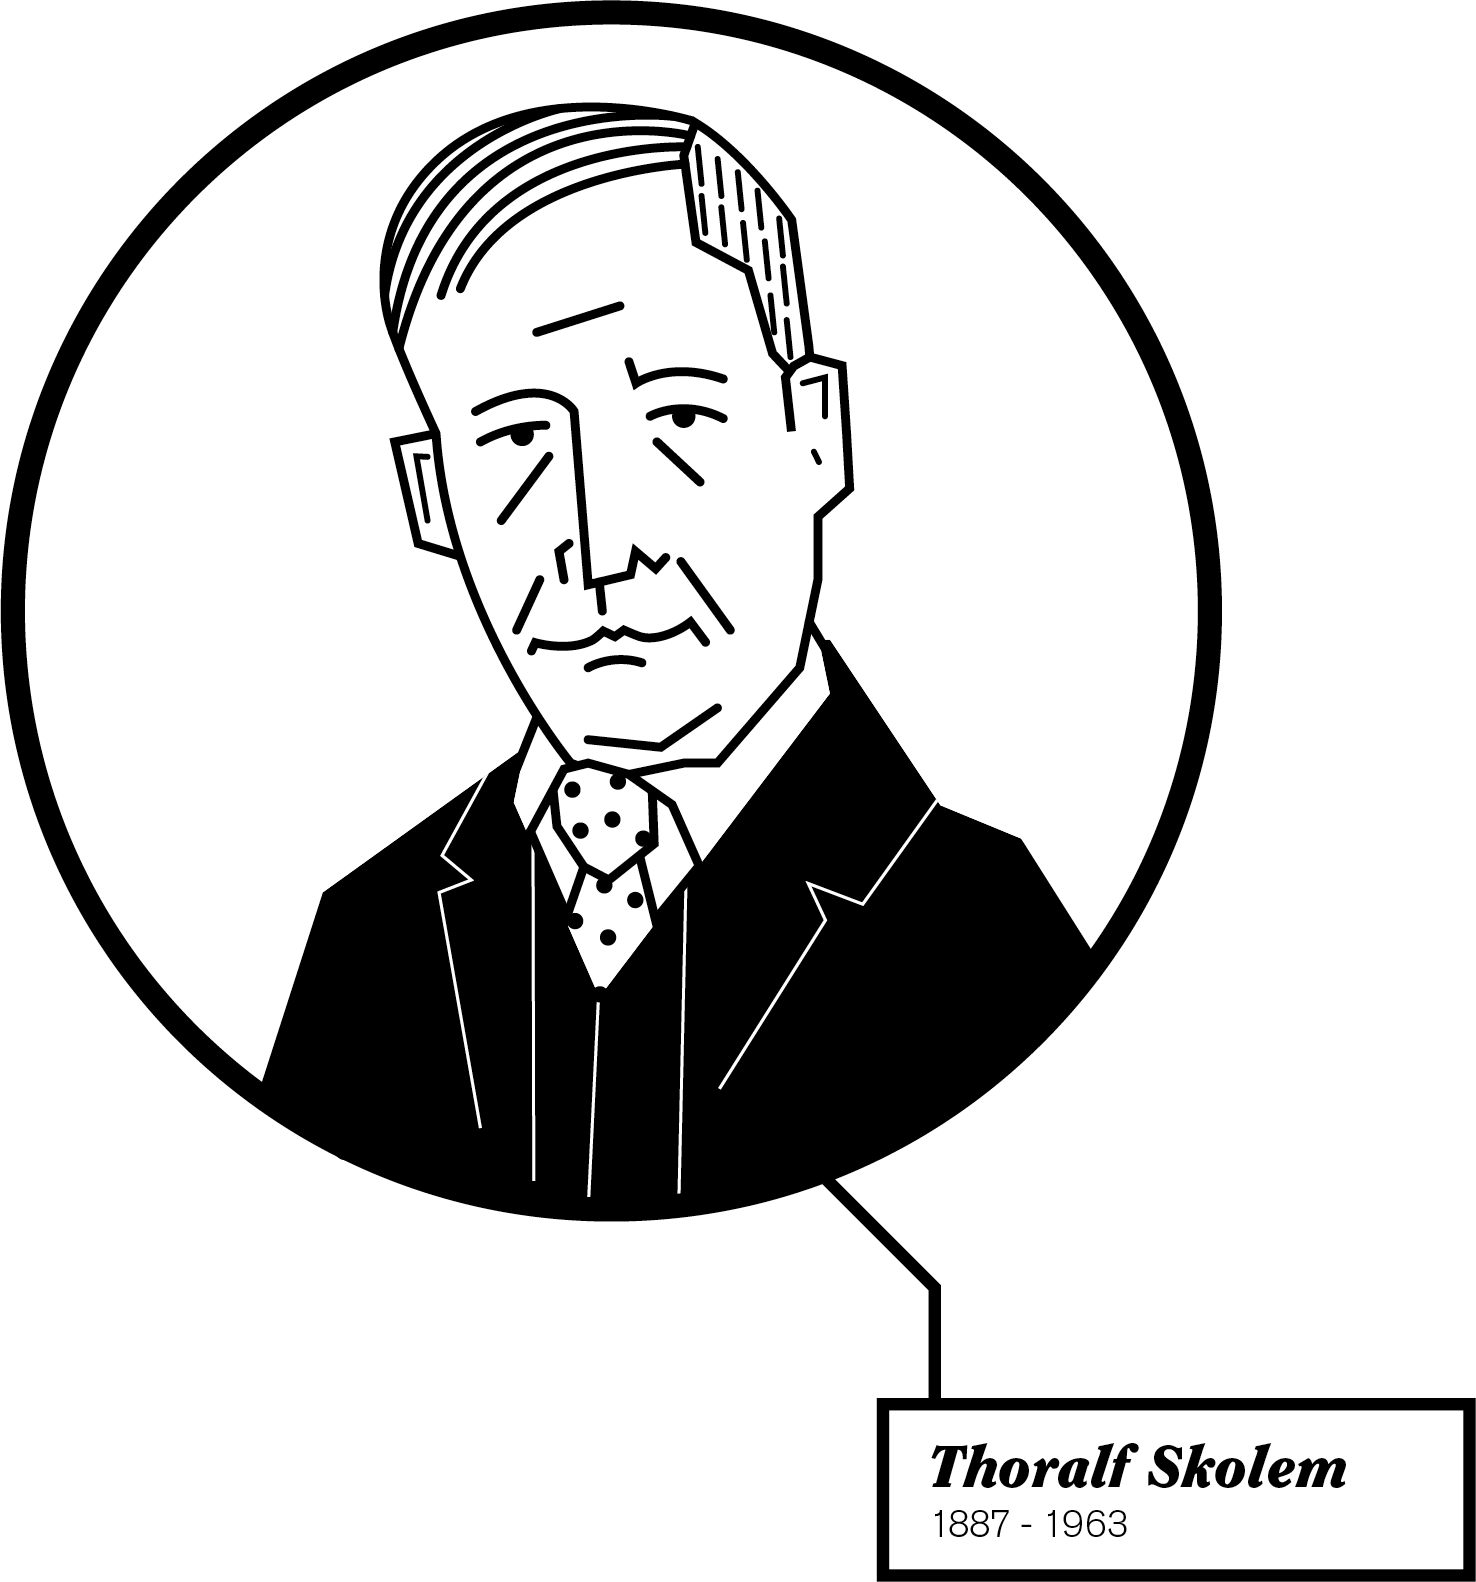
\includegraphics[width=\textwidth]{illustrations/SkolemChapter}
\vfill
\chapter{Pambuka}

Buku iki minangka pambuka metalogika, mligi kanggo mahasiswa ilmu komputer
lan filsafat. Jeneng “metalogika” nuduhaké disiplin kang nyinaoni logika
iku dhéwé. Logika ngrembug paugeran inferensi kang sah. Ing wujud simbolis
utawa formal, paugeran mau diandharaké nganggo basa formal, kayata basa
logika proposisional lan logika tataran kapisan. Metalogika nyelidiki sipat
basa-basa mau lan paugeran inferensi kang bener kang migunakaké basa iku.
Kita nyinaoni kepriyé mènèhi teges kang pas marang ungkapan ing basa formal,
kepriyé mbeneraké paugeran inferensi kang sah, lan apa waé sipat sistem
!!{derivation}, kalebu sipat komputasiné. Pitakonan iki wigati amarga basa
lan sistem !!{derivation} kasebut dienggo ing akèh widang, mligi matématika,
filsafat, ilmu komputer, lan linguistik. Pitakonan mau uga mènèhi tuladha
cara nyinaoni sistem formal kanthi umum. Saliyane basa logika kang
dirembug ing kéné, ana akèh basa liya kang narik kawigatèn. Para ahli
linguistik lan filsuf, upamané, nyinaoni basa kang luwih ruwet tinimbang
basa logika proposisional lan logika tataran kapisan. Para ahli ilmu
komputer uga nyinaoni \emph{jinis} basa liya, kayata basa pamrograman.
Cara mènèhi semantik, mbuktèkaké asil, lan nyelidiki sipat basa formal kang
dirembug ing kéné bisa ditrapaké ing kasus-kasus mau.

Kaya disiplin liyané, metalogika nduwèni kumpulan asil utawa fakta lan
kumpulan cara lan tèknik. Buku iki ngrembug kalorone. Akèh mahasiswa
bisa waé mung mbutuhaké sawatara asil saka buku iki ing njaba kuliah,
nanging bakal migunakaké cara kang dienggo kanggo mbuktèkaké asil mau.
Upamané, teorema L\"owenheim--Skolem arang tinemu ing ilmu komputer,
nanging cara kanggo mbuktèkaké teorema iku kerep dienggo. Akèh asil
liyané uga ana gegayutané karo rembugan tartamtu ing filsafat ngèlmu
lan metafisika. Mahasiswa filsafat bisa waé ora perlu mbuktèkaké asil
mau ing njaba kuliah iki, nanging kudu mangertèni tegesé. Pangertèn
kang tenanan mbutuhaké pamikiran tumrap definisi lan bukti kang
netepaké asil kasebut. Iki sapérangan alesan ngapa asil lan cara ing
buku iki dianjuraké, lan kadhang diwajibaké, kanggo mahasiswa ilmu
komputer lan filsafat.

Materi iki kapérang dadi telung pérangan. \Olref[sfr][][]{part}
ngrembug teori himpunan. Ing sajarahé, logika lan metalogika gegayutan
raket karo landhesan matématika. Landhesan matématika ngrembug kepriyé
objèk matématika kayata wilangan wutuh, rasional lan riil, fungsi, lan
ruwang bisa dipahami ing tataran paling dhasar. Teori himpunan mènèhi
salah siji wangsulan, lan ana uga wangsulan liya. Mula, teori
himpunan lan logika wis suwé disinaoni bebarengan. Himpunan, relasi,
lan fungsi tinemu ing manéka panaliten formal ing matématika, ilmu
komputer, lan pérangan filsafat kang luwih tèknis. Istilah-istilah iki
perlu kanggo ngrumusaké lan mbuktèkaké asil ing semantik, teori bukti,
lan landhesan komputabilitas. Upamané, kita bakal ngrembug himpunan
ungkapan, relasi konsèkuènsi lan kabisan dibuktèkaké, interpretasi
simbol predikat kang awujud relasi, fungsi kang bisa dikomputasi, lan
manéka relasi lan konstruksi kang migunakaké kabèh iku. Simbol
cekakan bisa nggampangaké andharan. Kita uga perlu mangertèni sipat
umum himpunan, relasi, lan fungsi. Yèn durung kulina mikir sacara
matématis lan ngrumusaké bukti, pérangan kapisan bisa dianggep
papan gladhi. Definisi dhasar bakal diwènèhaké, banjur dienggo ing
bukti kang saya ruwet. Mligi ing pérangan kapisan, mangertèni bukti
lan bisa nemokaké sarta ngrumusaké bukti dhéwé bisa luwih wigati
tinimbang mangertèni asilé waé. Yèn cara mikir matématis isih anyar,
tlitinen tuladha lan coba garapen soal-soalé.

Pérangan kapisan mbuktèkaké siji asil wigati, yaiku teorema Cantor.
Asil iki adhedhasar salah siji tuladha analisis konsèp kang paling
nggumunaké ing ngèlmu, yaiku analisis Cantor ngenani tanpa wates.
Sajroning pirang-pirang abad, tanpa wates mbingungaké para ahli
matématika lan filsuf. Sadurungé Cantor, durung ana cara kang trep
kanggo mangertèni tanpa wates. Akèh wong malah nganggep pamikiran
ngenani koleksi tanpa wates minangka kaluputan, amarga gagasané
dianggep ora runtut. Cantor nggawé tanpa wates bisa ditliti kanthi
runtut. Dhèwèké ngrembakakaké teori koleksi tanpa wates lan wilangan
tanpa wates kang bisa dienggo ngukur gedhéné koleksi mau. Cantor
nuduhaké yèn tanpa wates nduwèni tataran kang béda-béda. Teori
wilangan “transfinit” iki éndah lan ruwet. Buku iki ngrembug nganti
bisa nuduhaké tataran kang béda mau, yaiku tataran tanpa wates kang
bisa dietung lan kang ora bisa dietung. Asil iki nduwèni kagunan
wigati lan patut dimangertèni para ahli matématika, ahli ilmu
komputer, lan filsuf.

Ing \olref[fol][][]{part}, kita sinau logika tataran kapisan. Kita
bakal nemtokaké basané lan semantiké, yaiku apa kang diarani struktur
tataran kapisan lan kapan ukara tataran kapisan bener ing sawijining
struktur. Saka kéné kita bisa nindakaké rong bab wigati.
(1)~Kita bisa nemtokaké kanthi pas sacara matématis kapan sawijining
ukara dadi konsèkuènsi logis saka ukara liya. (2)~Kita bisa nliti
kepriyé relasi ing sawijining struktur tataran kapisan diciriaké déning
ukara kang bener ing struktur iku. Iki nuntun marang cara aksiomatis,
yaiku cara migunakaké ukara ing basa tataran kapisan kanggo mènèhi ciri
jinis struktur tartamtu. Sabanjuré kita ngrembug teori bukti lan
nyinaoni kalkulus sekèn lan dedhuksi alami ing wujud wiwitané,
kaya kang ditetepaké Gerhard Gentzen ing taun 1930-an. Yèn dosèn
milih salah siji sistem waé, tembung “!!{derivation}s” lan
“!!{derivability}” ing kuliah iku tumuju ing sistem kang dipilih.
Konsèkuènsi semantis lan !!{derivability} sintaktis iku rong cara kang
béda kanggo mènèhi teges kang pas marang gagasan yèn sawijining ukara
bisa diturunaké saka ukara liya. Teorema kesahihan lan kejangkeping
sistem nyambungaké loro gagasan mau. Mligi, kita bakal mbuktèkaké
teorema jangkepé G\"odel. Yèn sawijining ukara minangka konsèkuènsi
semantis saka sawatara ukara liya, ukara mau uga !!{derivable} saka
ukara-ukara kasebut. Rumusan kang ekuivalen yaiku mangkéné. Yèn
sawijining kumpulan ukara konsisten, yaiku ora ana kontradiksi kang bisa
dibuktèkaké saka kumpulan iku, ana sawijining struktur kang ndadèkaké
kabèh ukara mau bener.

Rumusan kapindho teorema jangkep iki bisa uga luwih nggumunaké.
Nalika G\"odel mbuktèkaké asil iki ing taun 1929, ahli matématika
Jerman David Hilbert misuwur amarga panemuné yèn konsistènsi, yaiku
bebas saka kontradiksi, wis cukup kanggo anané objèk matématika.
Kanthi tembung liya, manawa ahli matématika bisa mènèhi andharan kang
runtut bab sawijining struktur utawa kelas struktur, dhèwèké wenang
pracaya yèn struktur kuwi ana. Nalika semana akèh wong nganggep
panemu iki ora lumrah. Miturut wong-wong mau, kasunyatan yèn
andharan bab sawijining struktur ora ngandhut kontradiksi durung
njamin struktur mau ana. Nanging iki pancèn isi teorema jangkepé
G\"odel. Saliyane bab kang katon paradoksal lan narik kawigatèn sacara
filosofis iki, teorema jangkep nduwèni rong kagunan wigati. Kita bisa
mbuktèkaké asil luwih lanjut ngenani anané struktur kang ndadèkaké
ukara-ukara tartamtu bener. Rong asil kasebut yaiku teorema
kompaktitas lan teorema L\"owenheim--Skolem.

Ing \olref[tur][][]{part}, kita nggandhèngaké logika karo
komputabilitas. Gegayutan iki uga ana sajarahé. David Hilbert
ngajokaké masalah dhasar ing logika, yaiku golèk cara mekanis kang,
kanggo sembarang ukara logika, bisa mutusaké apa ana buktiné. Cara
mangkono ana kanggo logika proposisional. Cukup priksa kabèh tabel
kabeneran. Amarga cacahé winates, cara iku pungkasané mènèhi wangsulan
kang bener. Cara kang langsung kaya mangkono ora bisa ditrapaké
marang logika tataran kapisan, amarga cacah struktur kang bisa ana
tanpa wates, lan strukturé dhéwé bisa tanpa wates. Para ahli logika
nyoba pirang-pirang taun golèk cara kang luwih trep. Pungkasané
Alonzo Church lan Alan Turing mbuktèkaké yèn cara mangkono ora ana.
Kanggo mbuktèkaké iki, dhisik perlu definisi kang pas ngenani apa
kang diarani cara mekanis sacara umum. Yèn ana usul prosedur
kaputusan, mesthiné kita bisa wanuh yèn cara iku èfèktif. Kanggo
mbuktèkaké yèn ora ana cara èfèktif, kita kudu ndhisiki nganggo
definisi “cara èfèktif” lan saka kono mènèhi bukti kamustahilan.
Turing nglakoni iki. Dhèwèké ngajokaké gagasan mesin
Turing\footnote{Turing dhéwé ora mènèhi jeneng mangkono.} minangka
modèl matématis kanggo apa kang bisa ditindakaké déning prosedur
mekanis ing prinsipé. Iki tuladha liyané saka \emph{analisis
konsèp} informal kanthi piranti matématis. Wigatiné tumrap ilmu
komputer bisa dibandhingaké karo wigatiné analisis Cantor ngenani
tanpa wates tumrap matématika. Pakaryan utama ing pungkasan buku iki
yaiku mbuktèkaké rong teorema kamustahilan. Kita bakal nuduhaké yèn
“masalah mandheg” ora bisa dirampungi déning mesin Turing. Banjur
kita bakal nuduhaké yèn “masalah kaputusan” Hilbert kanggo logika
uga ora bisa dirampungi.

Buku iki sipaté matématis amarga ngrembug definisi matématis lan
mbuktèkaké asil kanthi cara matématis. Kawruh matématika kang jembar
ora dadi prasyarat. Buku iki ora mbutuhaké kawruh aljabar,
trigonometri, utawa kalkulus. Buku iki uga disusun supaya pamaca
ora kudu wis kulina karo cara matématika. Salah siji ancasé pancèn
\emph{ngrembakakaké} kaprigelan nalar lan mbuktèkaké kang dibutuhaké
kanggo mangertèni lan mbuktèkaké asil. Susunan buku manut konvensi
matématika amarga konvensi iku njaga kajelasan lan katliten.
Upamané, wigati kanggo ngerti kapan sawijining pratelan minangka
kesimpulan argumen, kapan minangka alesan kanggo pratelan liya, lan
kapan minangka pambuka tembung anyar. Mula, kita mènèhi tetenger
“definisi” kanggo pérangan kang nepungaké istilah utawa simbol anyar.
Asil utawa panemon diwènèhi tetenger “teorema”, “proposisi”,
“lema”, utawa “korolari”. Saliyane manut konvensi mau, kita
migunakaké cara bukti logis kang bisa uga wis dikenal saka kuliah
logika kapisan. Cara \emph{induksi} uga kerep dienggo kanggo
mbuktèkaké asil. Rong bab ing lampiran ngrembug cara-cara bukti iki.

\paragraph{Cathetan kanggo dosèn}
Materi buku iki trep kanggo kuliah logika formal tingkat kapindho
sajroning sasemèster. Ing Logic~II ing University of Calgary, aku
ngajar materi iki sajroning 12 minggu kanthi rincian kang luwih
winates tinimbang buku iki. Upamané, lumrahé aku mung ngrembug
dedhuksi alami lan ora ngrembug kanthi rinci bukti jangkep kanggo
logika mawa identitas. Mahasiswa wis mèlu Logic~I, kang lumrahé
nganggo \emph{\href{https://forallx.openlogicproject.org}{forall x:
Calgary}}. Buku iku migunakaké paugeran dedhuksi alami kang padha,
nanging ing format Fitch.

Vèrsi paling anyar buku asli ana ing
\href{https://slc.openlogicproject.org}{slc.openlogicproject.org}
kanthi format PDF lan kerep owah. Lisènsi CC BY maringi hak kanggo
ngundhuh lan mbagekaké buku iki dhéwé. Supaya kabèh mahasiswa nganggo
vèrsi kang padha sajroning semester, unggahna PDF kang dipilih ing
sistem manajemen pasinaon lan wènèhana mahasiswa akses menyang berkas
iku. Toko buku kampus uga kena nyithak PDF. Sawetara toko buku bisa
tuku lan nyetok buku sampul alus kang didol liwat Amazon.

Sintaksis, semantik, lan sistem bukti logika tataran kapisan didhukung
déning \emph{Carnap} (\href{https://carnap.io}{carnap.io}), piranti
pasinaon logika daring gratis anggitané Graham Leach-Krouse. Carnap
bisa kanggo nglumpukaké lan mriksa soal kanthi otomatis, kayata
!!{derivation}s dedhuksi alami lan kalkulus sekèn, mènèhi struktur
kanggo teori prasaja, lan gladhi nulis simbol. Ana uga simulator mesin
Turing ing \href{https://turing.openlogicproject.org}{turing.openlogicproject.org}
kanggo nggambaraké materi ing \olref[tur][][]{part}. Tuladha-tuladha
wis cumepak ing simulator iku.


\cleartoverso
\thispagestyle{empty}
\ \vfill
\noindent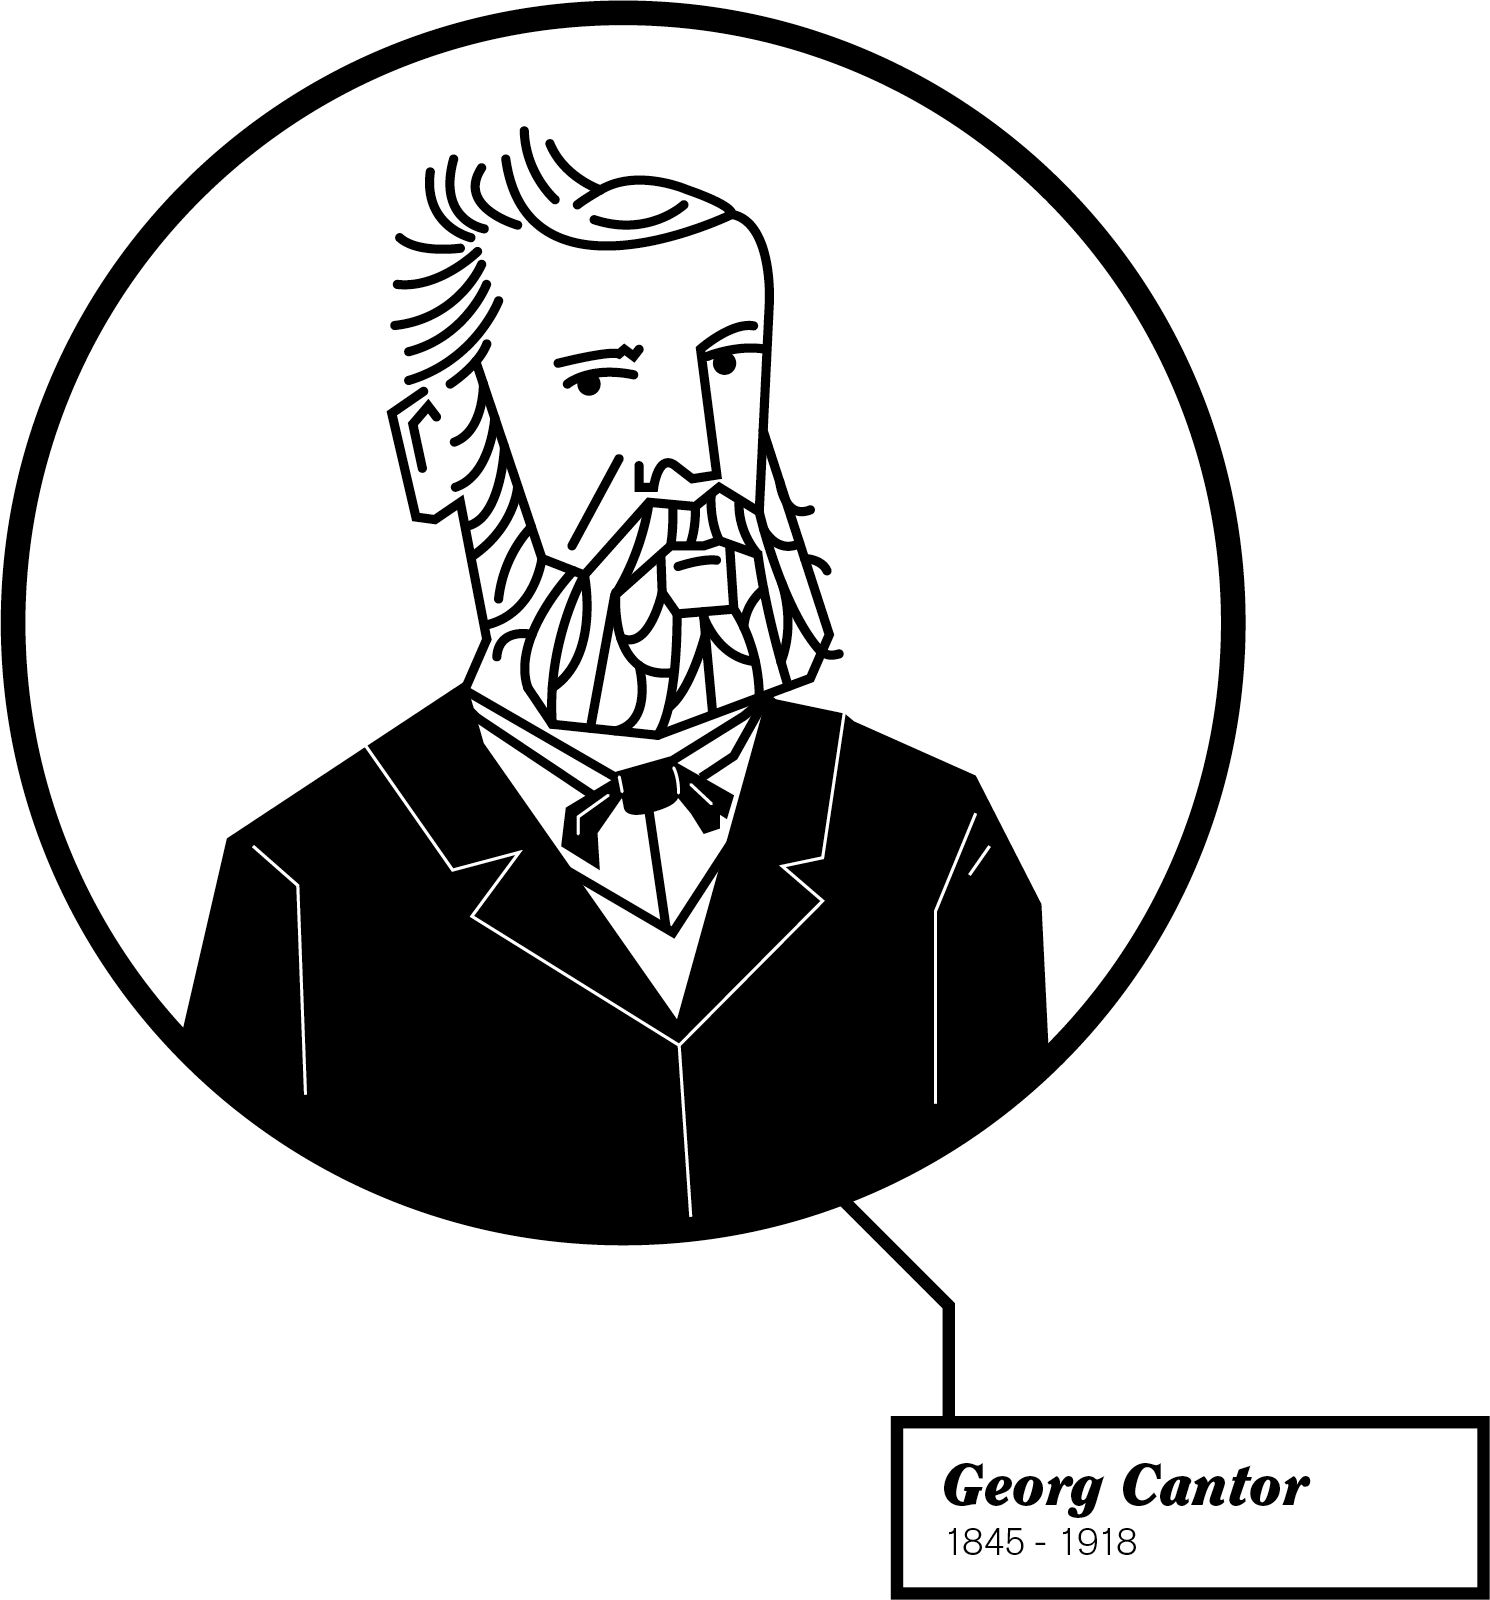
\includegraphics[width=\textwidth]{illustrations/CantorChapter}
\vfill
\mainmatter
\olimport*[sets-functions-relations]{sets-functions-relations}

\cleartoverso
\ifodd\value{page}\stepcounter{page}\fi
\thispagestyle{empty}
\ \vfill
\noindent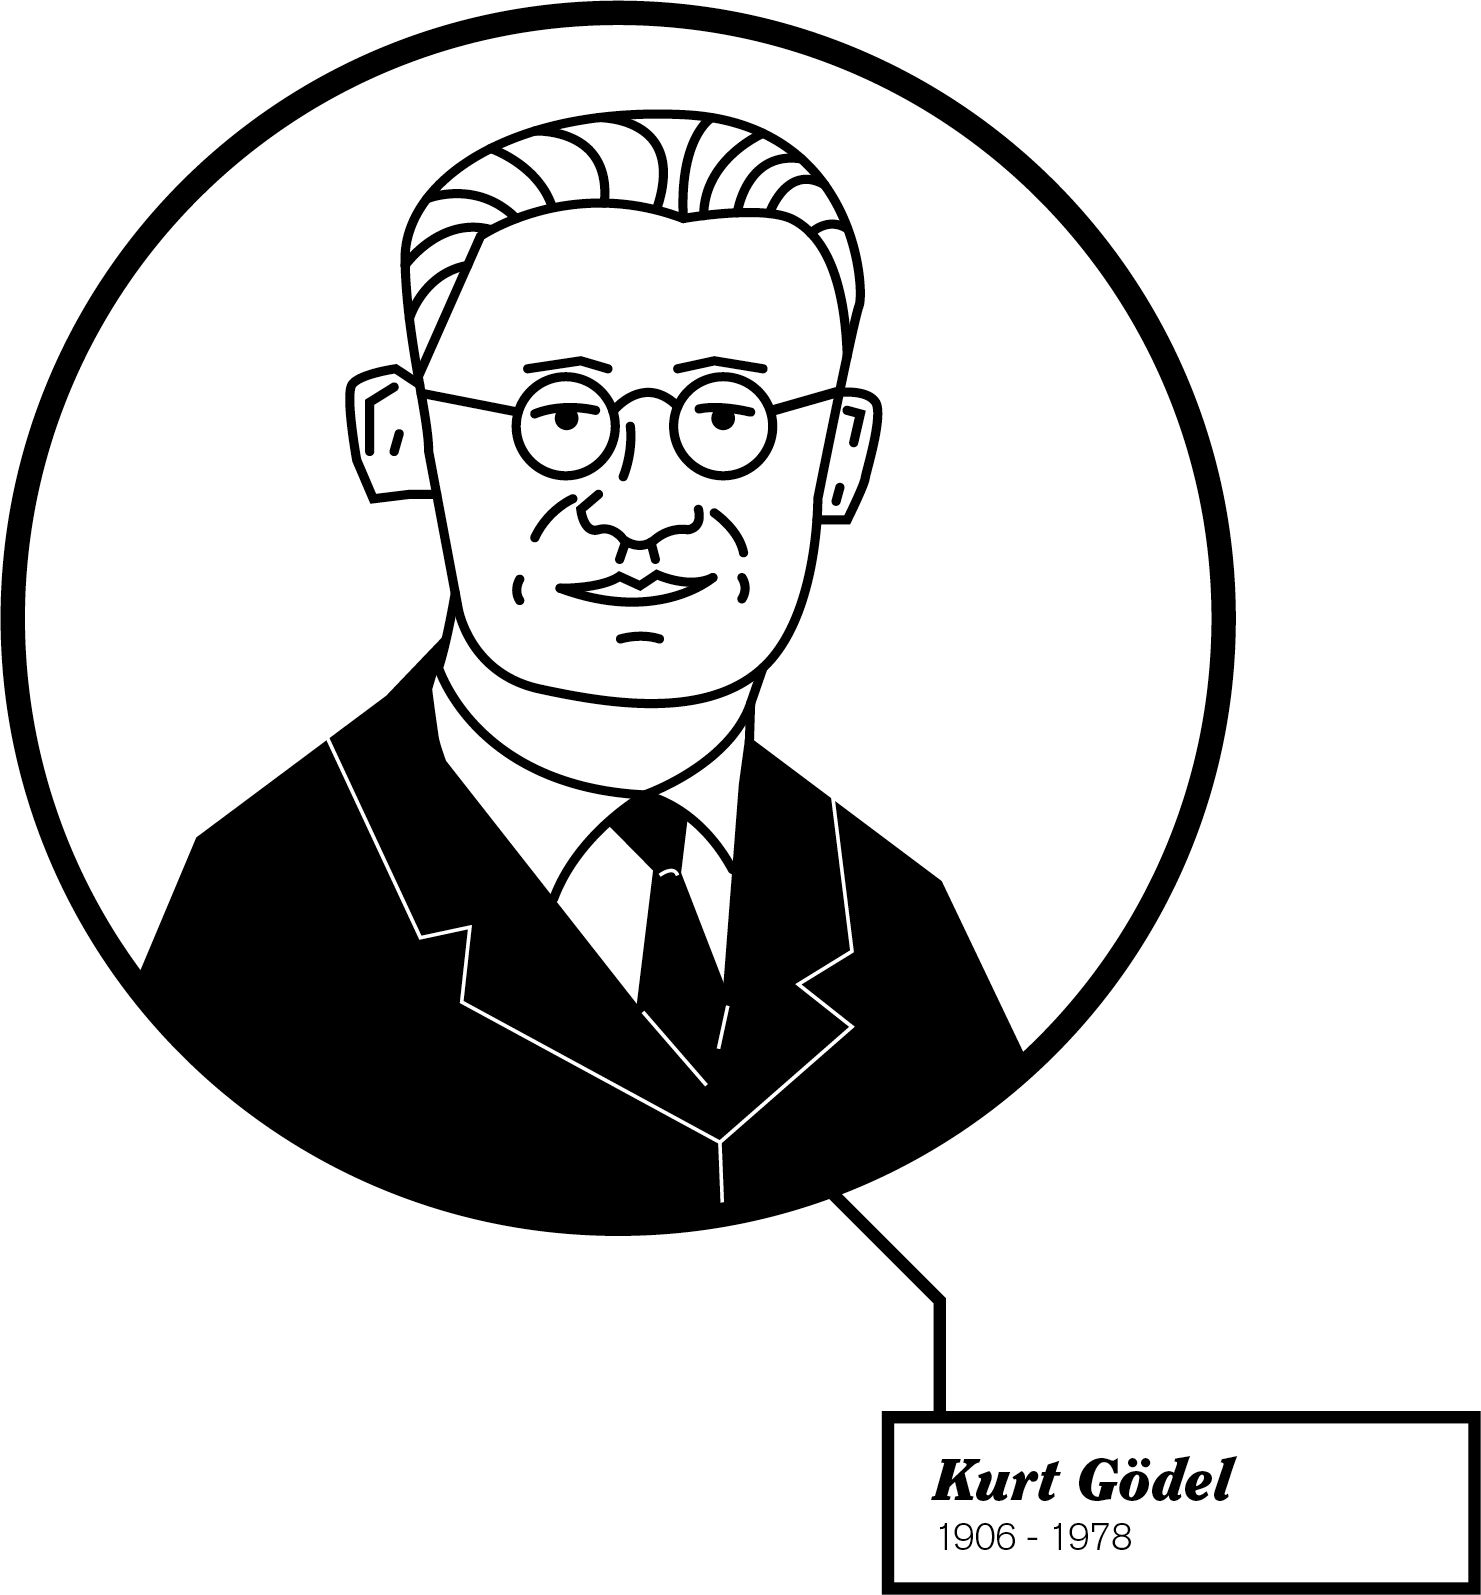
\includegraphics[width=\textwidth]{illustrations/GodelChapter}
\vfill
\olimport*[first-order-logic]{first-order-logic}

\cleartoverso
\ifodd\value{page}\stepcounter{page}\fi
\thispagestyle{empty}
\ \vfill
\noindent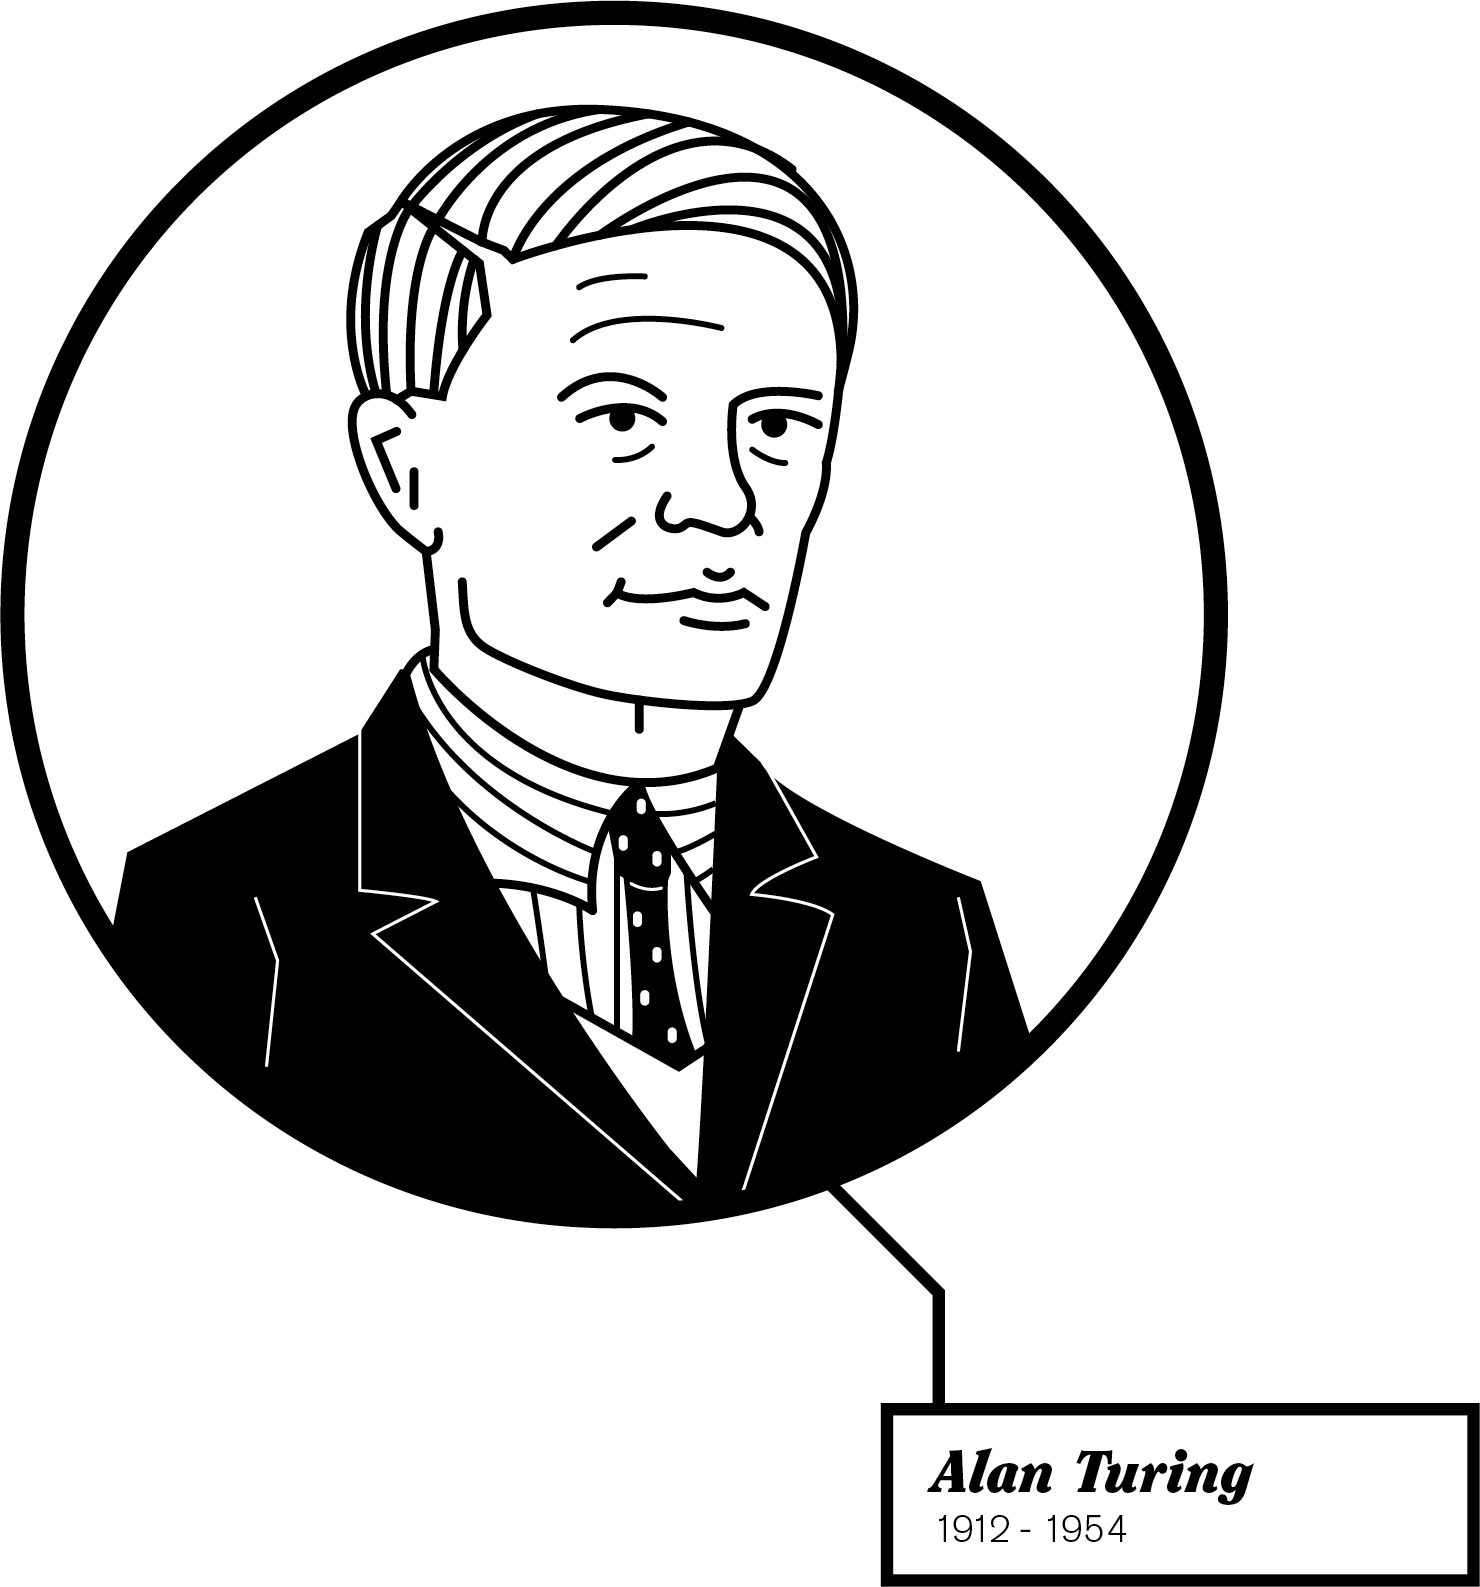
\includegraphics[width=\textwidth]{illustrations/TuringChapter}
\vfill
\olimport*[turing-machines]{turing-machines}

\cleartoverso
\ifodd\value{page}\stepcounter{page}\fi
\thispagestyle{empty}
\ \vfill
\noindent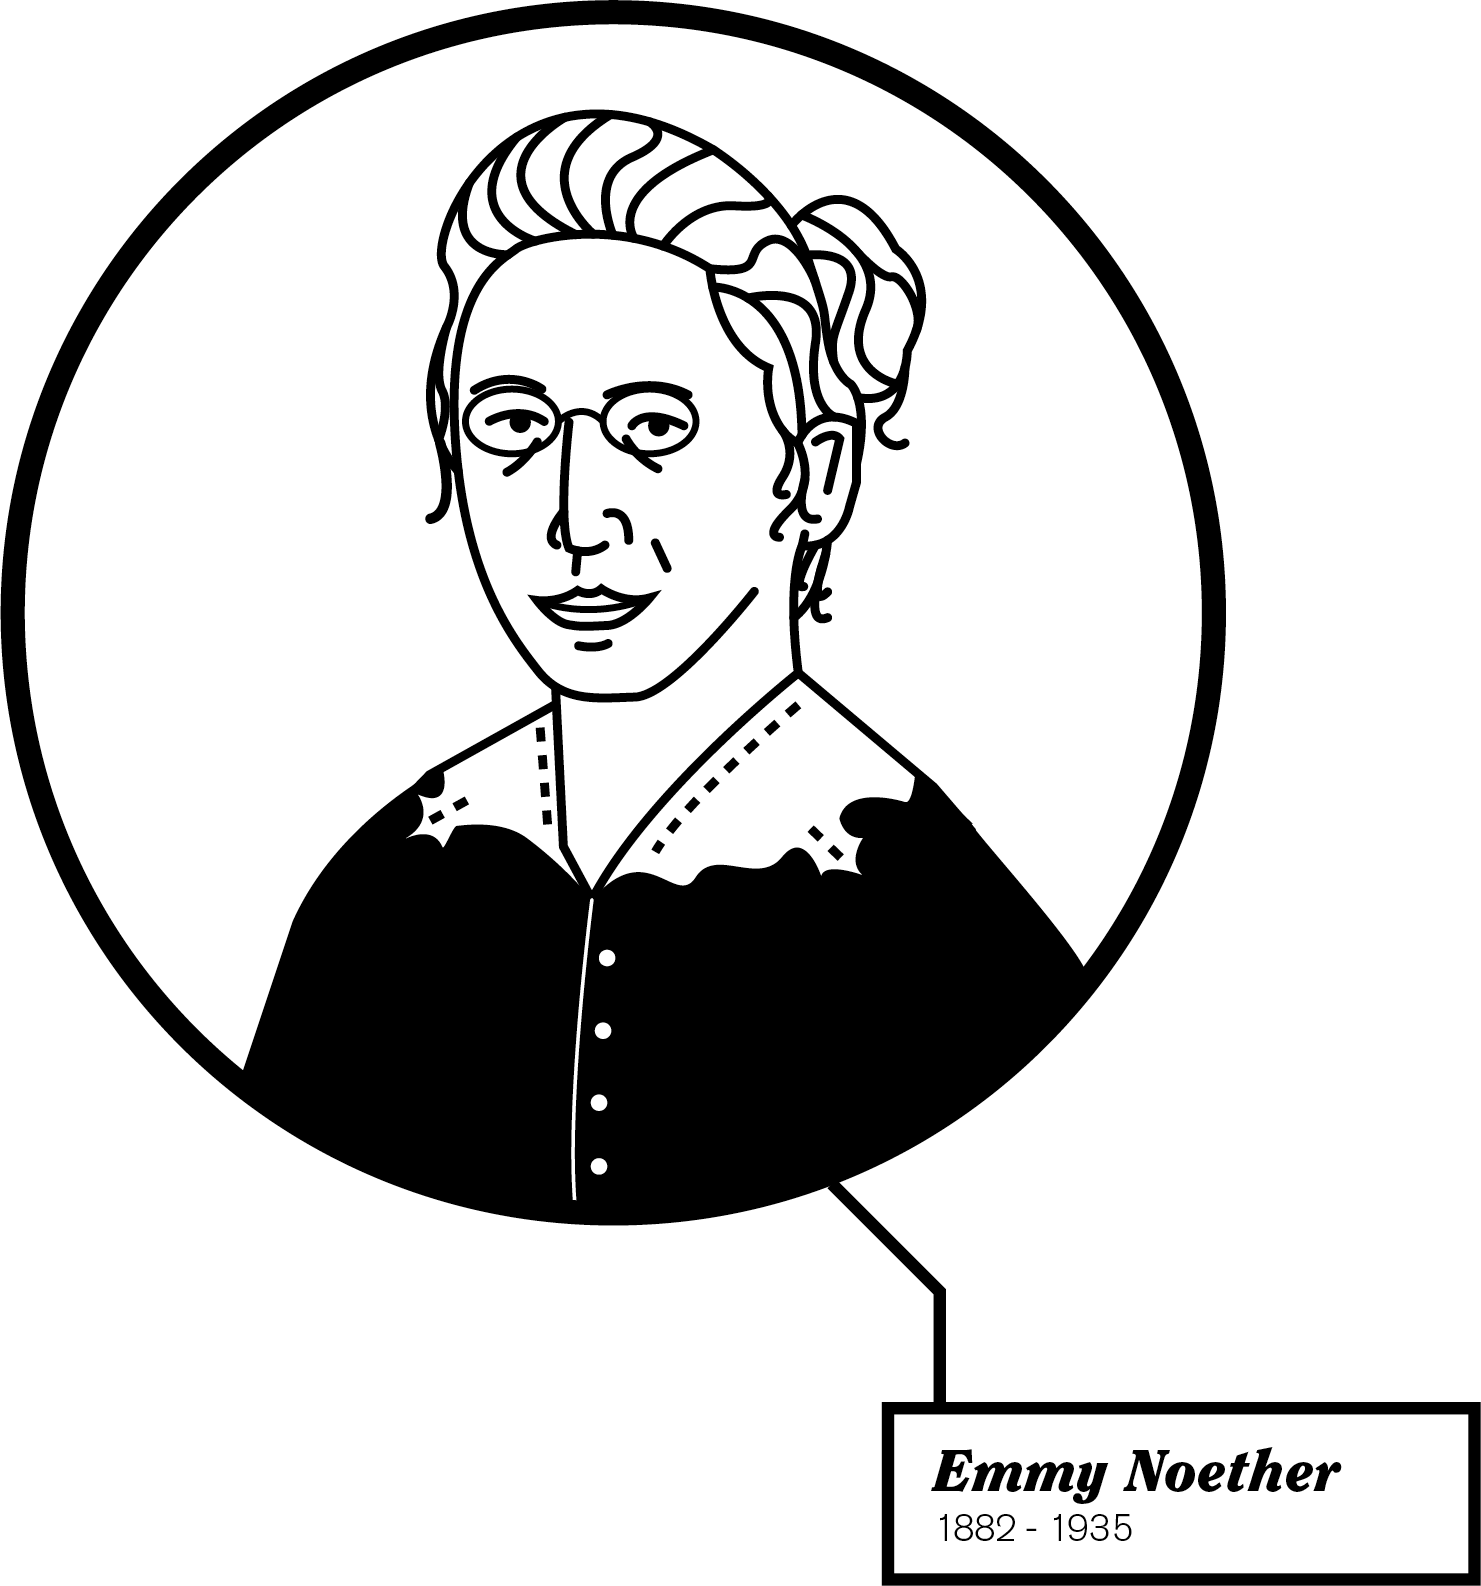
\includegraphics[width=\textwidth]{illustrations/NoetherChapter}
\vfill
\appendix
\olimport*[methods/proofs]{proofs}
\olimport*[methods/induction]{induction}

\stopproblems
\def\ifproblems#1{}
\def\figurename{Gambar}
\setlength{\olphotowidth}{.45\textwidth}
\chapter{Babad Para Ahli Logika}
\olimport*[history/biographies]{georg-cantor}
\olimport*[history/biographies]{alonzo-church}
\olimport*[history/biographies]{gerhard-gentzen}
\olimport*[history/biographies]{kurt-goedel}
\olimport*[history/biographies]{emmy-noether}
\olimport*[history/biographies]{bertrand-russell}
\olimport*[history/biographies]{alfred-tarski}
\olimport*[history/biographies]{alan-turing}
\olimport*[history/biographies]{ernst-zermelo}
\olimport*[reference/greek-alphabet]{greek-alphabet}

\glsaddall
\printglossary[title=Glosarium,toctitle=Glosarium]
\clearpage
\photocredits
\bibliographystyle{natbib-oup}
\bibliography{\olpath/bib/open-logic}
\olimport*{\olpath/locale/\ollangid/content/open-logic-about}

\end{document}
